%\documentclass[a4paper,12pt]{report}
\documentclass[a4paper,12pt]{extreport}

\bibliographystyle{iopart-num}
\usepackage{amsmath}
%\usepackage{citesort}
\usepackage{subfigure}
\usepackage{graphicx}
\graphicspath{{fig/}}
\usepackage{ifpdf}
\ifpdf\usepackage{epstopdf}\fi
\usepackage[export]{adjustbox}
\usepackage[numbers]{natbib}

\def\apj{ApJ}
\def\apjl{ApJ Lett.}
\def\mnras{MNRAS}
\def\nat{Nature}
\def\physrevB{Phys. Rev. B}
\def\prd{Phys. Rev. D}
\def\prl{Phys. Rev. Lett.}
\def\pre{Phys. Rev. E}
\def\araa{Ann. Rev. Astron. Astrophys.}                % "Ann. Rev. Astron. Astrophys."
\def\aap{Astron. Astrophys.}                  % "Astron. Astrophys."
\def\aaps{Astron. Astrophys. Suppl. Ser.}                 % "Astron. Astrophys. Suppl. Ser."
\def\aj{Astron. J.}                      % "Astron. J."
\def\apjs{Astrophys. J. Suppl. Ser.}                  % "Astrophys. J. Suppl. Ser."
\def\pasp{Publ. Astron. Soc. Pac.}                  % "Publ. Astron. Soc. Pac."
\def\apjl{ApJ Lett.}                   % letter at ApJ
\def\pasj{PASJ}
\def\apss{Astroph. Space Sci.}
\def\aplett{Astroph. Lett.}
\def\ssr{Space Sci. Rev.}
\def\jcap{J. Cosmol. Astropart. Phys.}
\def\apspr{Sov. Sci. Rev. Sect. E}
\def\nar{New Astron. Rev.}
\def\aapr{ Astron. Astrophys. Rev.}

\begin{document}
	\title{On X-ray emission from Fast Blue Optical Transients}
	
	\author{A M Bykov$^{1}$, V I Romansky$^{1}$}
	

Recent observations of Fast Blue Optical Transients \cite{Margutti2019, Ho2019cow,Ho2020koala,Coppejans2020, Ho2021at2020, YaoAt2020mrf} show high level of X-ray radiation. There are suggested different scenarios of  origins of this radiation: central engine or interaction of shock with external medium. In this paper we present model of interaction of shock with strong wind from close star, producing X-ray emission via inverse compton scattering on the photons of this star. This assumption is supported by studying of local environment of object AT2018cow \cite{SunAT2018environment} showing that there are two young massive stur clusters in vicinity of AT2018cow. Young massive star clusters (YMSC) have a lot of stars with strong winds and high luminocity in rather small volume (f. e. cluster Westerlund-1 has 6 yellow giants, 4 red supergiants, 24 Wolf-Rayet stars, and dozens of OB stars in the radius of 1 parsec \cite{Clark2005westerlund, Crowther2006westerlund, Negueruela2010westerlund}). So if supernova explosion happens in YMSC, it is probable that ejecta will interact with strong wind of neighbour star, placed at distance about $10^{17}  cm$.  In this work we use object CSS161010, decribed in \cite{Coppejans2020}, because it has very high ejecta velocity ($0.3 c - 0.5 c$) and it makes Particle-in-Cell (PIC) modeling of particle acceleration, which we use to obtain distribution function of emitting electrons, more simple??. This paper is organized as follows: in section \ref{synchrotron} we evaluate synchrotron radio flux from CSS161010 and fit it to observation data, varying such hydrodynamical parameters as magnetic field and number density. In section \ref{hydrodynamic} we present hydrodinamic simulation of interaction between supernova ejecta and stellar wind, using parameters obtained on previous step. And in section \ref{compton} we evaluate Inverse Compton X-ray flux from the region beyond wind bow-shock.

\section{synchrotron radiation}\label{synchrotron}
Observations of radio flux from CSS16101 \cite{Coppejans2020} shows that it's spectrum is consistent with synchrotron self-absorption model. Method of analytical estimations of source parameters for this case was developed in works \cite{Chevalier1998, ChevalierFransson} and is commonly used to analyze spectrums of FBOTs \cite{Ho2019cow, Ho2020koala, Coppejans2020, Ho2021at2020}. But this approach needs an assumption of power-law distribution of electrons. In this work we use electrons distribution function obtained from PIC simulations of shock wave and evaluate synchrotron radiation using numerical integration of standard formulae for emissivity and absorption coefficient, described in \cite{Ginzburg1975, Ghisellini}.

Distribution function of emitting electrons is evaluated using PIC simulation with code SMILEI \cite{Derouillat}. Setups for shock simulation is decribed in details in our previous work \cite{BykovUniverse}. Shock was initialized due to collision of uniform plasma flow with velocity $0.3 c$ with reflecting wall. Magnetiztion was $\sigma = B^2/4 \pi m_p \gamma c^2 = 0.002$ and diffirent inclination angles of magnetic field were studied. One can see the well-known effect, that efficiency of particle acceleration strongly depends on the magnetic obliquety to the shock \cite{SironiSpitkovsky2009pair, Crumley2019, GuoSironi2014_1, Romansky2018} on the figure \ref{distributions}, where electron distributions in the shock downstream for different inclination angles are shown.


\begin{figure}[h!]
	\centering
	\begin{minipage}{0.48\textwidth}
		\centering
		\includegraphics[width=0.98\textwidth]{./fig/distributions.png} 
		\caption{Electron distribution function in the downstream of shock with different inclination angles $\theta$}
		\label{distributions}
	\end{minipage}\hfill
	\begin{minipage}{0.48\textwidth}
		\centering
		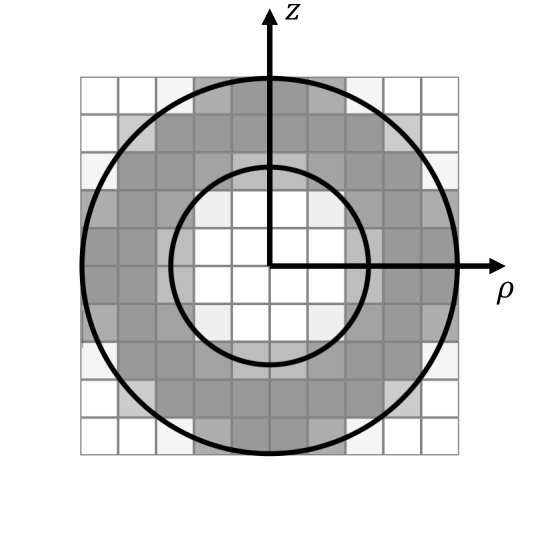
\includegraphics[width=0.98\textwidth]{./fig/sphericalSource.png} 
		\caption{Scheme of numerical model of spherical radiation source}
		\label{sphericalSource}
	\end{minipage}
\end{figure}

For evaluating radiation we use our numerical code FAINA, which allows to evaluate synchrotron and inverse compton radiation and also fit model to observational data. Radiation source in the code is presented as spherical layer in cylindrical coordinates as schematically shown on figure \ref{sphericalSource}. Direction to observer is along z-axis. Colour shows the part of volume of cell is filled with emitting plasma. Each cell has it's own magnetic field, electron number density and distribution. This geometry allows to integrate emissivty along line of sight, taking into account self-absorption.

Analytical analysis \cite{Coppejans2020} and numerical modeling \cite{BykovUniverse} shows that magnetic field in the system should be rather strong (about $0.3 G$ at distances about $10^{17} cm$). It does not seems to be possible that quasiuniform interstellar magnetic field can be so strong. Another option is to use magnetic field generated by the star, but on this distances it should be perpendicular to the shock velocity \cite{Parker} and particle can not be accelerated in quasiperpendicular shocks, as it was mentioned above. So we assumed presence of strong turbulence around the star, containing $90 \%$ of magnetic energy, wtih characteristic scale about radius of expanding ejecta, and Kolmogorov's energy spectum. Due to fluctuating magnetic field, shock become quasiparallel at some points, and can be a source of accelerated particles. Time of forming the powerlaw tail of electrons distribution in our PIC simulations is much smaller than time of significant changes of shock magnetic obliquety in this large-scale turbulence, and we assume that electron distribution becomes stationar in every cell of emitting envelope and corresponds to the inclination angle of magnetic field at this point. Number density of electrons is considered uniform inside the radiation source.


With this model of radiation source we fit evaluated synchrotron radiation to observational data of radio flux from CSS161010 at 98 day after explosion (the first observation when both radio and X-ray flux was detected), and derive such parameters as mean magnetic field, concentration and width of the spherical shell. Our best fit for radio flux and observational data are shown on Figure \ref{synchrotron}. Evaluated parameters are magnetic field $B = 0.6 G$, number density $n = 50000{cm}^{-3}$ and shell width $l = 0.01\cdot R = 1.4E15 cm$. This parameters are consistent with results of other authors \cite{Coppejans2020}, only electrons number density is much higher because of not-powerlaw distribution. 
\begin{figure}
	\centering
	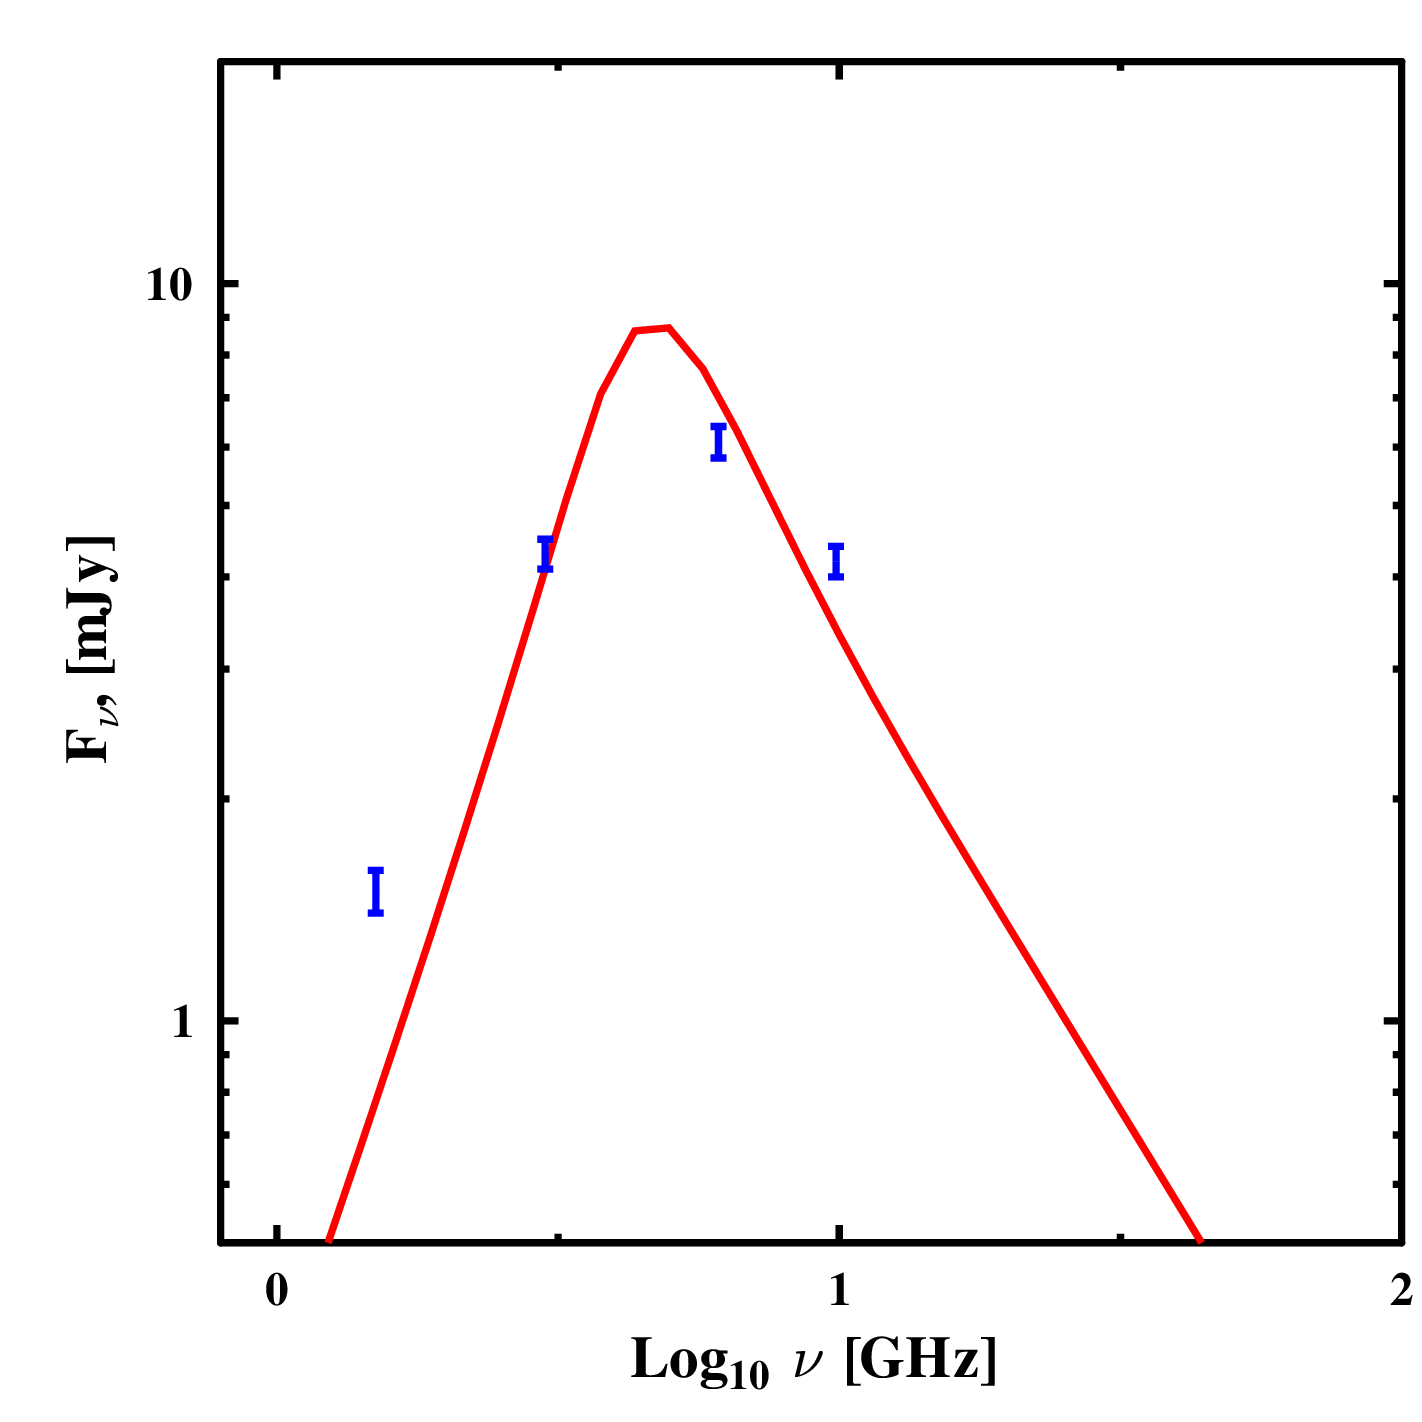
\includegraphics[width=0.5\textwidth]{./fig/radiation2.png} 
	\caption{Observed and modeled radiospectrum of CSS161010 at 98 day after explosion.}
	\label{synchrotron}
\end{figure}

And then we use obtained parameters for hydrodynamical modeling of interection between sub-relativistic ejecta and strong stellar wind from neighbour star.
%написать почему не хватает комптона от всей оболочки
\section{hydrodynamic}\label{hydrodynamic}
In our model we took two close stars, on a distance $1.4\cdot10^{17} cm$, wich corresponds to the radius of expanding shock of CSS161010 at 98 day after explosion. It is  possible in young massive star clusters where are a lot of bright stars with powerfull stellar winds (OB, Wolf-Rayet, and red supergiants) in the small volume. We will refer to them as first star - stable, generating wind, and the second - exploded as supernova. We assumed both stars have winds with velocity $v_w = ?$ and mass loss $\dot{M} = 10^{-5} M_\odot $ per year and luminocity $L=500000 L_\odot$ and surfece temperature $T = 2.5\cdot10^6 K$ which is typical for Wolf-Rayet stars. The magnetic fied of the wind is initialized using \cite{}, and for the first star  it's amplitude is $100 G$ at the radius $10$ while for the second we need much stronger field to satisfy synchrotron observational data. So we took magnetic field $1000 G$ at the radius $10^{12}$, stars with such strong fields are described in \cite{}.

For hydrodinamcal simulation we use code PLUTO \cite{MignonePluto}. We used several nested setups on different scales. At first we performed 3d modeling of two stable stars with parameters described above until they winds form a stable configuration. First star is placed at point with coordinates $x_1 = 0, y_1 = 0, z_1 = 0$, and the second at point with $x_2 = 0, y_2 = 0, z_2 = 1.4\cdot10^{17} cm$. Plane x-y is equatorial plane of winds of both stars. Sizes of the simulation box are $Lx = 6\cdot 10^{17} cm$ and $Ly = Lz = 3\cdot 10^{17}$ with number of grid points 400, 200 and 200 respectively. The next step was 1d spherical modeling of second star explosion. We use ejecta mass $M_{ej} = 0.1 M_\odot$ and velocity $v_{ej} = 0.3 c$ and initial conditions as described in \cite{ChevalierLiang1989, Petruk2021snr}. The simulation box is splitted into three regions - in the central region with radius $r_0 = ?$ density is constant and velocity is proportional to radius $v(r) = 0.3 c r/r_0$. In the next region between $r_0$ and $r_1 = 2 r_0$ number density depends on radius as $n(r) \propto r^{-9}$ and velocity is also proportional to radius. And in the last region with $r > r_1$ stellar wind with constant velocity $v_w$ and mass loss $\dot{M}$is initialized. Profiles of ejecta density at different time moments are shown on figure \ref{snr}.
\begin{figure}
	\centering
	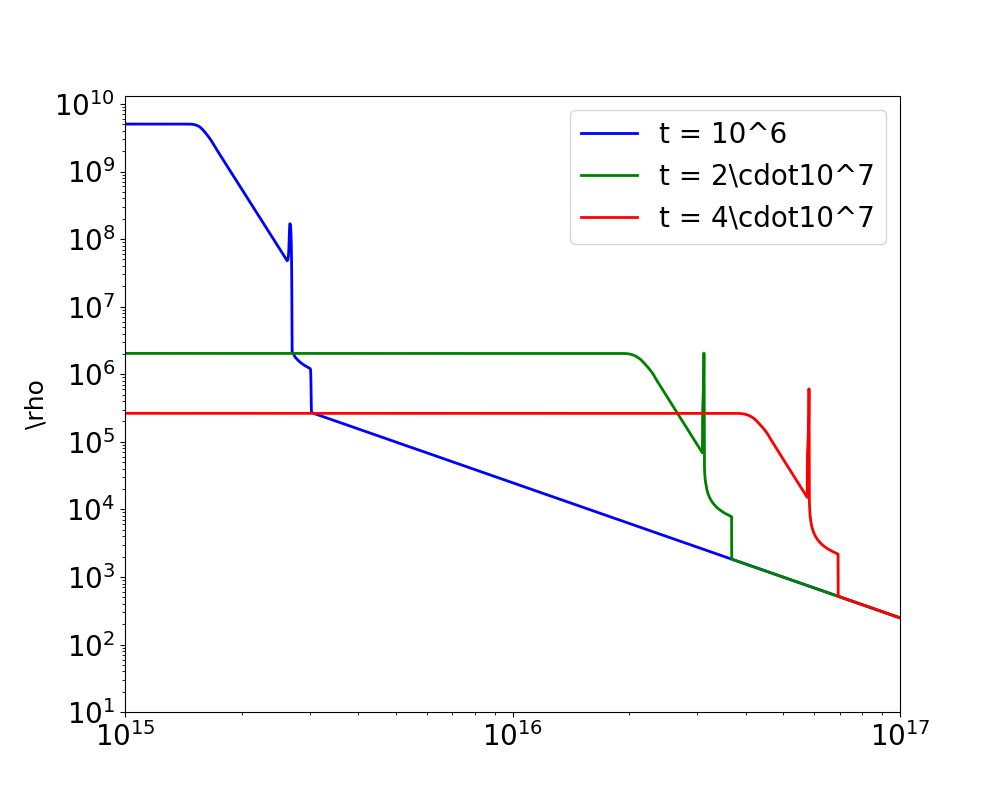
\includegraphics[width=0.5\textwidth]{./fig/snr.png} 
	\caption{Density profile of supernova explosion.}
	\label{snr}
\end{figure}

At the third step we simulated setup with smaller scale - with size $Lx = 1.05\cdot 10^{17} cm$ and $Ly = Lz = 0.9\cdot 10^{16}$ and combined results of the previous steps as initial conditions. Also results of 1d modeling were used as time-dependent boundary condition on the right boundary. And at the last step, in setup with the smallest scale $Lx = 0.3\cdot 10^{17} cm$ and $Ly = Lz = 1.5\cdot 10^{15}$, which is necessary to resolve bow- and tremination shock of the wind of the first star, we use results of the third step as initial and boundary conditions. Number density in different setups and their ierarchy scheme is shown on figure \ref{density}. On the panel a one can see iteraction of two winds in large-scale simulation at time before the explosion. On the panel b propagation of ejecta in middle-scale simulation at time $t_1 \approx 1.0\cdot10^7 s$ is shown. On the panel c one can see it in small-scale simulation at time $t_2 \approx 1.1\cdot10^7 s$. Ans on the panel d there is zoomed picture of wind bowshock in small-scale simulation at time $t_3 \approx 1.4\cdot10^7 s$ Magnetic field at the same time moments is shown on figure \ref{Bfield}.
\begin{figure}
	\centering
	\begin{minipage}{0.48\textwidth}
		\centering
		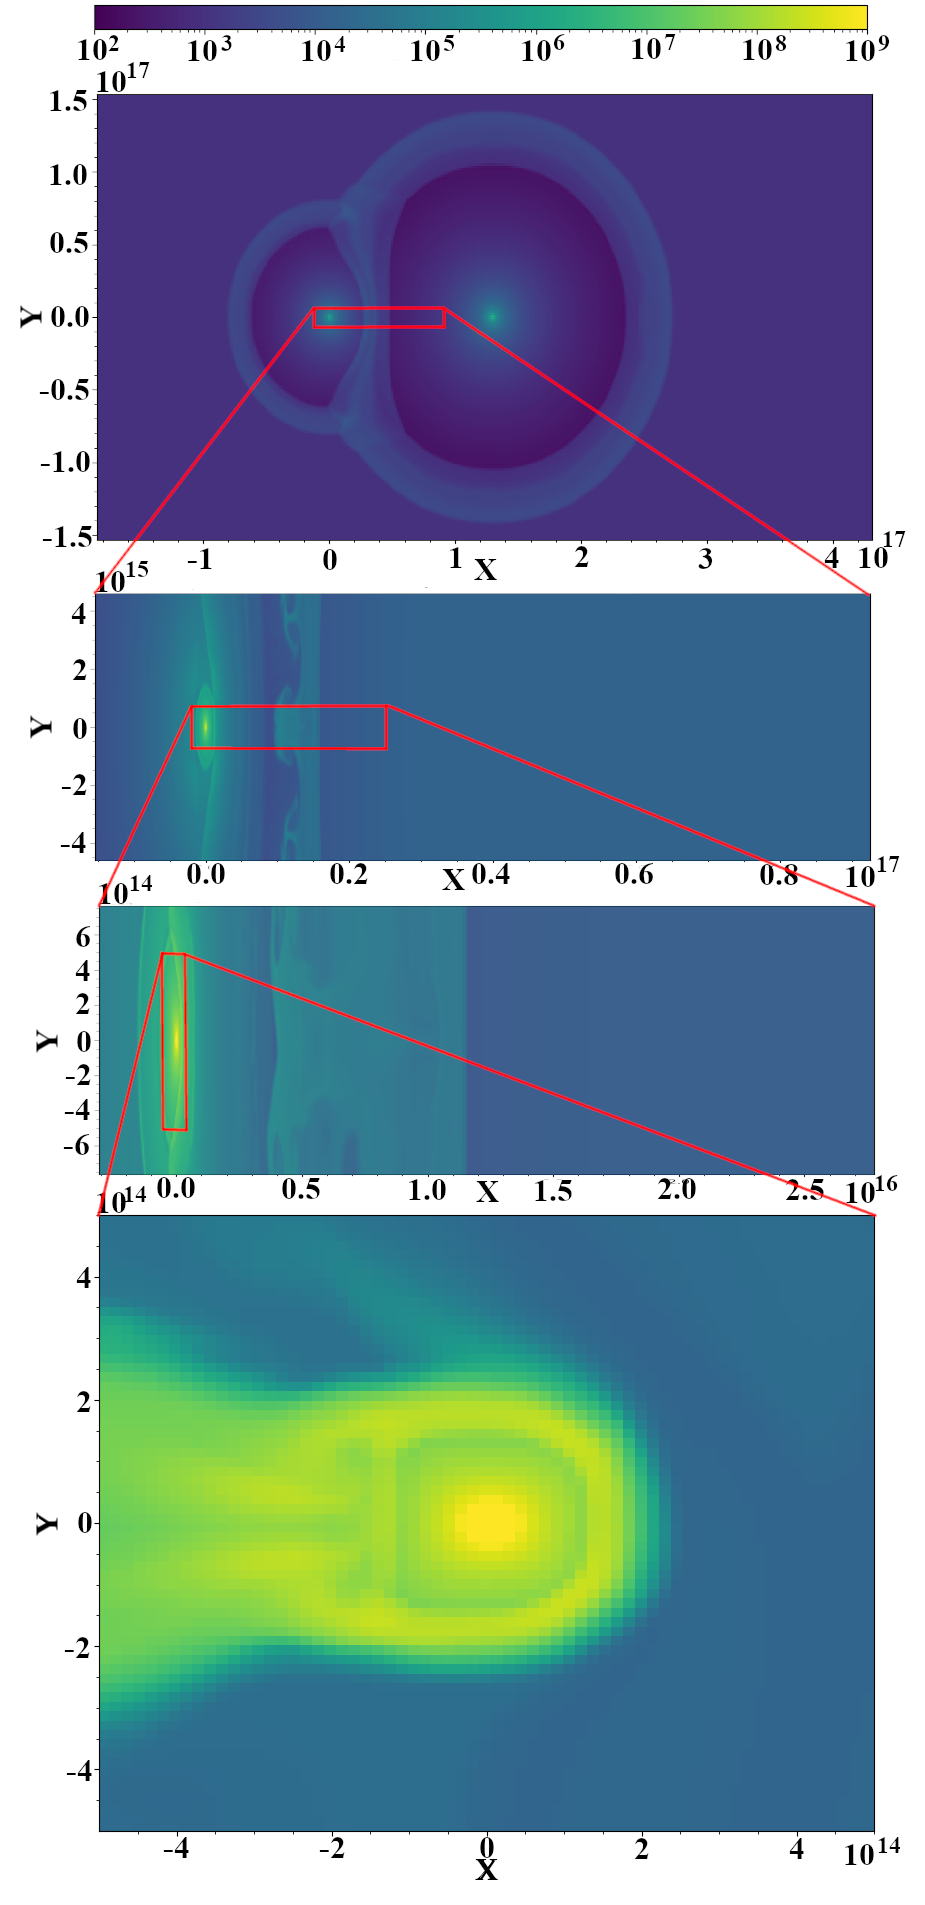
\includegraphics[width=0.98\textwidth]{./fig/density.png} 
		\caption{Density profile of the system at different time moments}
		\label{density}
	\end{minipage}\hfill
	\begin{minipage}{0.48\textwidth}
		\centering
		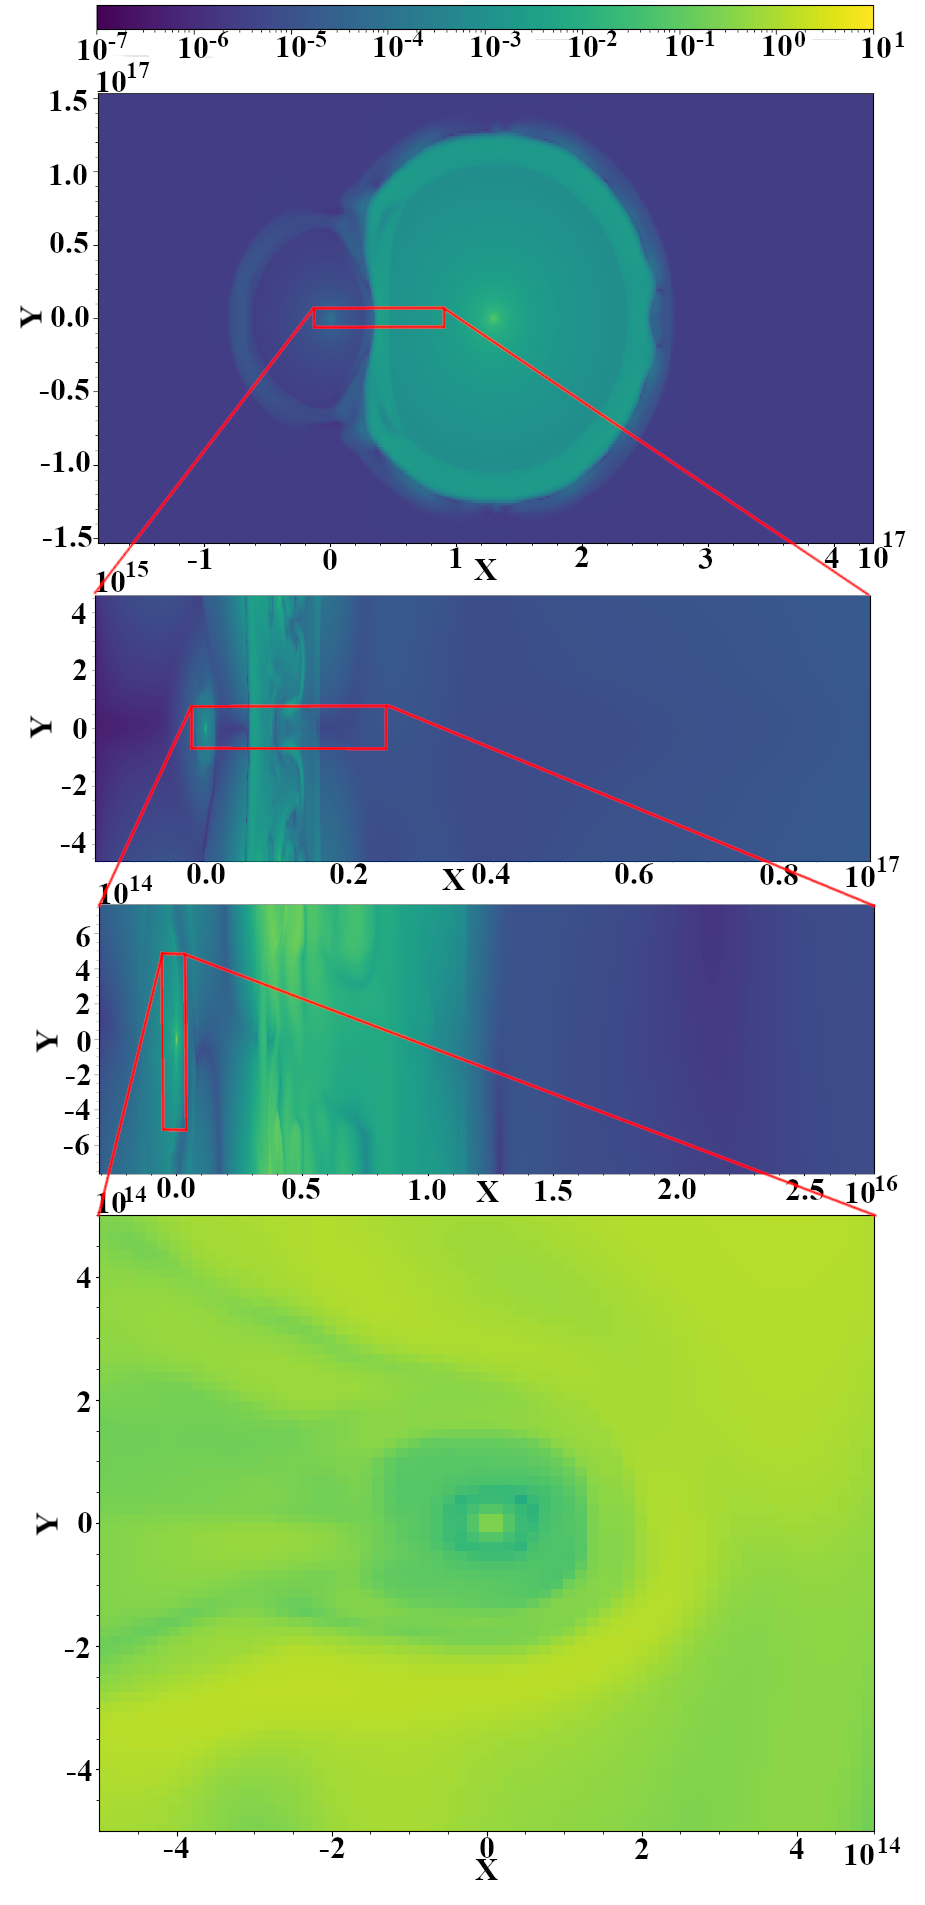
\includegraphics[width=0.98\textwidth]{./fig/Bfield.png} 
		\caption{Magnetic field profile of the system at different time moments}
		\label{Bfield}
	\end{minipage}
\end{figure}

Simulations showed that ejecta of supernovae, moving in interstellar medium has profile with thin and dense peak with number density $n \approx 10^5 cm^{-3}$ and width $d = 10^{16}$, and wide region with number density $\approx 10^4 cm^{-3}$ behind the peak.

The wind bow-shock has radius $R_w \approx 2\times10^{14} cm$ and number density $n_w \approx 10^9 cm^{-3}$. With this parameters, and luminocity and temperature of the star, one can estimate observed X-ray flux, produced by inverse compton scattering.
 
\section{Inverse compton radiation}\label{compton}

In our model X-ray flux is generated via inverse compton scattering in the region of iteraction between wind from the first star, and supernova ejecta from the second. Relativistic ejecta has huge bulk pressure and wind is compressed to small region with high number dencity. Also this region is close to high luminous star, and there are suitable conditions for strong inverse compton radiation. Electrons can be accelerated on the shock fronts or on the shearing flows. So electrons distribution function is 
%непонятно чт писать
We assume that source is a cylinder with radius $R_w$, and height also equals $R_w$, with axis oriendted along line of sight, and with uniform number density $n_w$. 
and photons distribution corresponds to the radiation of the first star at distance $R_w$. With this parameter modeled X-ray flux in the energy range $0.3-10 keV$ is $F_m = $ which is consistent with observed flux of CSS161010 at 99 day after explosion $F_{obs = }$ \cite{Coppejans2020}.

\bibliographystyle{iopart-num}
\bibliography{fbotcompton}
\end{document}